\documentclass{article}

\usepackage[utf8x]{inputenc}
\usepackage[T1]{fontenc}
\usepackage{fullpage}
\usepackage{amsmath}
\usepackage{amssymb}
\usepackage{amsfonts}
\usepackage{pxfonts}
\usepackage{ucs}
\usepackage{hyperref}
\usepackage{xfrac}
\usepackage{lmodern}
\usepackage{graphicx}
\usepackage{multirow}
\usepackage{tikz}
\usepackage{pgfplots}
\usepackage{pgf}
\usetikzlibrary{patterns}

% Schreibweisen für bestimmte Überschriften:
%
%					Beispiele
% \section{große Überschrift} 		Folgen und Reihen
% \subsection{große Überschrift} 	Häufungspunkte und Grenzwerte von Folgen
% \paragraph{Definition}
% \paragraph{Schreibweise}
% \paragraph{Bemerkung}
% \paragraph{Bezeichnung}
% \paragraph{Satz}

\begin{document}

% zwischen den beiden folgenden kommentaren schreiben

% start
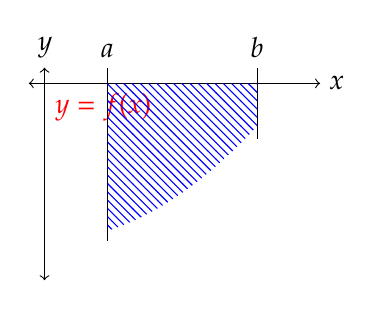
\begin{tikzpicture}[domain=-2:3.5]
	\draw[<->] (-0.2,0) -- (3.5,0) node[right] {$x$};
	\draw[<->] (0,-2.5) -- (0,0.2) node[above] {$y$};
	\draw[domain=0.5:3][color=red] plot[samples=100] function{0.2*(x)**2-2}
		node[below right] {$y=f(x)$};
	\draw (0.8,-2) -- (0.8,0.2) node[above] {$a$};
	\draw (2.7,-0.7) -- (2.7,0.2) node[above] {$b$};
	
 	\fill [pattern=north west lines, pattern color=blue, domain=0.8:2.7, variable=\x]
	  (0.8, 0)
	  -- plot ({\x}, {0.2*(\x)^2-2})
	  -- (2.7, 0)
	  -- cycle;
\end{tikzpicture}

$\int_a^b f(x)dx<0$\\

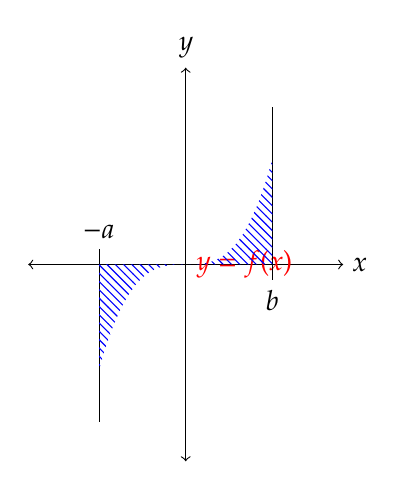
\begin{tikzpicture}[domain=3.5:-2.5]
	\draw[<->] (-2,0) -- (2,0) node[right] {$x$};
	\draw[<->] (0,-2.5) -- (0,2.5) node[above] {$y$};
	\draw[domain=-1.25:1.25][color=red] plot[samples=100] function{x**3}
		node[right] {$y=f(x)$};
	\draw (-1.1,-2) -- (-1.1,0.2) node[above] {$-a$};
	\draw (1.1,2) -- (1.1,-0.2) node[below] {$b$};
	
 	\fill [pattern=north west lines, pattern color=blue, domain=-1.1:1.1, variable=\x]
	  (-1.1, 0)
	  -- plot ({\x}, {(\x)^3})
	  -- (1.1, 0)
	  -- cycle;
\end{tikzpicture}

$\int_a^{-a} x^3dx=0$\\

\subsection{Numerische Integration}
meist äquidistante Zerlegung, d.h $\Delta x_i = x_i - x_{i-1}$ konstant für alle $i=1,...,n$
\subsection{Trapezformel}
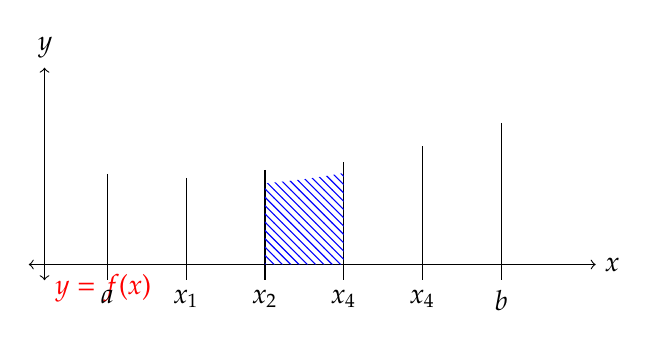
\begin{tikzpicture}[domain=-2:7]
	\draw[<->] (-0.2,0) -- (7,0) node[right] {$x$};
	\draw[<->] (0,-0.2) -- (0,2.5) node[above] {$y$};
	\draw[domain=0.5:6.5][color=red] plot[samples=100] function{0.05*(x-2)**2+1}
		node[below right] {$y=f(x)$};
	\draw (0.8,1.15) -- (0.8,-0.2) node[below] {$a$};
	\draw (1.8,1.1) -- (1.8,-0.2) node[below] {$x_1$};
	\draw (2.8,1.2) -- (2.8,-0.2) node[below] {$x_2$};
	\draw (3.8,1.3) -- (3.8,-0.2) node[below] {$x_4$};
	\draw (4.8,1.5) -- (4.8,-0.2) node[below] {$x_4$};
	\draw (5.8,1.8) -- (5.8,-0.2) node[below] {$b$};
	
 	\fill [pattern=north west lines, pattern color=blue, domain=2.8:3.8, variable=\x]
	  (2.8, 0)
	  -- plot ({\x}, {0.05*(\x -2)^2+1})
	  -- (3.8, 0)
	  -- cycle;
\end{tikzpicture}\\
Zerlegung des Intervalls $[a,b]$\\
$Z_n = \{ x_0^{(?)}, x_1^{(?)}, x_2^{(?)}, ..., x_n^{(?)}\}$\\
$x_0 = a, x_1 = b$\\
$x_0 < x_1 < x_2 < ... < x_{n-1} < x_n$\\
$\Delta x_i = x_i-x_{i-1}$ Intervallbreite\\
$\eta_n = \overset{max}{i=1,...n}\{\Delta x_i \}$ Feinheit der Zerlegung $Z_n$\\ % overset passt noch nicht ganz. alignment ist off
$\xi_i$ Zwischenpunkte, $x_{i-1} \leq \xi_i \leq x_i (i=1,...,n)$\\
Zwischensumme $S_n = \sum_{i=1}^{n}f(\xi_i)\Delta x_i$\\
$Z_{n+1}$ heißt Verfeinerung der Zerlegung $Z_n$ falls $Z_{n+1}\overset{>}{\neq}Z_n$\\
Existiert $S=\underset{\lim n}{\Rightarrow \infty}S_n$ %unabhängig $\eta_n \Rightarrow 0$\\
von der Zerlegung und der Wahl der Zwischenpunkte, so heißt\\
$\int_{a}^{b} f(x)dx= \underset{\lim}{n \Rightarrow \infty} \sum_{i=1}^{n}f(\xi_i)\Delta x_i$\\
bestimmtes Integral von f über das Intervall $[a,b]$
% stop

\end{document}
